% Options for packages loaded elsewhere
\PassOptionsToPackage{unicode}{hyperref}
\PassOptionsToPackage{hyphens}{url}
%
\documentclass[
]{article}
\usepackage{amsmath,amssymb}
\usepackage{lmodern}
\usepackage{iftex}
\ifPDFTeX
  \usepackage[T1]{fontenc}
  \usepackage[utf8]{inputenc}
  \usepackage{textcomp} % provide euro and other symbols
\else % if luatex or xetex
  \usepackage{unicode-math}
  \defaultfontfeatures{Scale=MatchLowercase}
  \defaultfontfeatures[\rmfamily]{Ligatures=TeX,Scale=1}
\fi
% Use upquote if available, for straight quotes in verbatim environments
\IfFileExists{upquote.sty}{\usepackage{upquote}}{}
\IfFileExists{microtype.sty}{% use microtype if available
  \usepackage[]{microtype}
  \UseMicrotypeSet[protrusion]{basicmath} % disable protrusion for tt fonts
}{}
\makeatletter
\@ifundefined{KOMAClassName}{% if non-KOMA class
  \IfFileExists{parskip.sty}{%
    \usepackage{parskip}
  }{% else
    \setlength{\parindent}{0pt}
    \setlength{\parskip}{6pt plus 2pt minus 1pt}}
}{% if KOMA class
  \KOMAoptions{parskip=half}}
\makeatother
\usepackage{xcolor}
\usepackage[margin=1in]{geometry}
\usepackage{color}
\usepackage{fancyvrb}
\newcommand{\VerbBar}{|}
\newcommand{\VERB}{\Verb[commandchars=\\\{\}]}
\DefineVerbatimEnvironment{Highlighting}{Verbatim}{commandchars=\\\{\}}
% Add ',fontsize=\small' for more characters per line
\usepackage{framed}
\definecolor{shadecolor}{RGB}{248,248,248}
\newenvironment{Shaded}{\begin{snugshade}}{\end{snugshade}}
\newcommand{\AlertTok}[1]{\textcolor[rgb]{0.94,0.16,0.16}{#1}}
\newcommand{\AnnotationTok}[1]{\textcolor[rgb]{0.56,0.35,0.01}{\textbf{\textit{#1}}}}
\newcommand{\AttributeTok}[1]{\textcolor[rgb]{0.77,0.63,0.00}{#1}}
\newcommand{\BaseNTok}[1]{\textcolor[rgb]{0.00,0.00,0.81}{#1}}
\newcommand{\BuiltInTok}[1]{#1}
\newcommand{\CharTok}[1]{\textcolor[rgb]{0.31,0.60,0.02}{#1}}
\newcommand{\CommentTok}[1]{\textcolor[rgb]{0.56,0.35,0.01}{\textit{#1}}}
\newcommand{\CommentVarTok}[1]{\textcolor[rgb]{0.56,0.35,0.01}{\textbf{\textit{#1}}}}
\newcommand{\ConstantTok}[1]{\textcolor[rgb]{0.00,0.00,0.00}{#1}}
\newcommand{\ControlFlowTok}[1]{\textcolor[rgb]{0.13,0.29,0.53}{\textbf{#1}}}
\newcommand{\DataTypeTok}[1]{\textcolor[rgb]{0.13,0.29,0.53}{#1}}
\newcommand{\DecValTok}[1]{\textcolor[rgb]{0.00,0.00,0.81}{#1}}
\newcommand{\DocumentationTok}[1]{\textcolor[rgb]{0.56,0.35,0.01}{\textbf{\textit{#1}}}}
\newcommand{\ErrorTok}[1]{\textcolor[rgb]{0.64,0.00,0.00}{\textbf{#1}}}
\newcommand{\ExtensionTok}[1]{#1}
\newcommand{\FloatTok}[1]{\textcolor[rgb]{0.00,0.00,0.81}{#1}}
\newcommand{\FunctionTok}[1]{\textcolor[rgb]{0.00,0.00,0.00}{#1}}
\newcommand{\ImportTok}[1]{#1}
\newcommand{\InformationTok}[1]{\textcolor[rgb]{0.56,0.35,0.01}{\textbf{\textit{#1}}}}
\newcommand{\KeywordTok}[1]{\textcolor[rgb]{0.13,0.29,0.53}{\textbf{#1}}}
\newcommand{\NormalTok}[1]{#1}
\newcommand{\OperatorTok}[1]{\textcolor[rgb]{0.81,0.36,0.00}{\textbf{#1}}}
\newcommand{\OtherTok}[1]{\textcolor[rgb]{0.56,0.35,0.01}{#1}}
\newcommand{\PreprocessorTok}[1]{\textcolor[rgb]{0.56,0.35,0.01}{\textit{#1}}}
\newcommand{\RegionMarkerTok}[1]{#1}
\newcommand{\SpecialCharTok}[1]{\textcolor[rgb]{0.00,0.00,0.00}{#1}}
\newcommand{\SpecialStringTok}[1]{\textcolor[rgb]{0.31,0.60,0.02}{#1}}
\newcommand{\StringTok}[1]{\textcolor[rgb]{0.31,0.60,0.02}{#1}}
\newcommand{\VariableTok}[1]{\textcolor[rgb]{0.00,0.00,0.00}{#1}}
\newcommand{\VerbatimStringTok}[1]{\textcolor[rgb]{0.31,0.60,0.02}{#1}}
\newcommand{\WarningTok}[1]{\textcolor[rgb]{0.56,0.35,0.01}{\textbf{\textit{#1}}}}
\usepackage{graphicx}
\makeatletter
\def\maxwidth{\ifdim\Gin@nat@width>\linewidth\linewidth\else\Gin@nat@width\fi}
\def\maxheight{\ifdim\Gin@nat@height>\textheight\textheight\else\Gin@nat@height\fi}
\makeatother
% Scale images if necessary, so that they will not overflow the page
% margins by default, and it is still possible to overwrite the defaults
% using explicit options in \includegraphics[width, height, ...]{}
\setkeys{Gin}{width=\maxwidth,height=\maxheight,keepaspectratio}
% Set default figure placement to htbp
\makeatletter
\def\fps@figure{htbp}
\makeatother
\setlength{\emergencystretch}{3em} % prevent overfull lines
\providecommand{\tightlist}{%
  \setlength{\itemsep}{0pt}\setlength{\parskip}{0pt}}
\setcounter{secnumdepth}{-\maxdimen} % remove section numbering
\ifLuaTeX
  \usepackage{selnolig}  % disable illegal ligatures
\fi
\IfFileExists{bookmark.sty}{\usepackage{bookmark}}{\usepackage{hyperref}}
\IfFileExists{xurl.sty}{\usepackage{xurl}}{} % add URL line breaks if available
\urlstyle{same} % disable monospaced font for URLs
\hypersetup{
  pdftitle={DataVisualization},
  hidelinks,
  pdfcreator={LaTeX via pandoc}}

\title{DataVisualization}
\author{}
\date{\vspace{-2.5em}2024-02-06}

\begin{document}
\maketitle

\hypertarget{a-gapminder-plot}{%
\section{A Gapminder Plot}\label{a-gapminder-plot}}

\hypertarget{the-basic-plot-can-be-created-with-ggplot-and-aesthetic-mappings}{%
\paragraph{1. The basic plot can be created with ggplot and aesthetic
mappings:}\label{the-basic-plot-can-be-created-with-ggplot-and-aesthetic-mappings}}

\begin{Shaded}
\begin{Highlighting}[]
\NormalTok{gm2007 }\OtherTok{\textless{}{-}} \FunctionTok{filter}\NormalTok{(gapminder, year }\SpecialCharTok{==} \DecValTok{2007}\NormalTok{)}
\FunctionTok{ggplot}\NormalTok{(gm2007) }\SpecialCharTok{+}
  \FunctionTok{geom\_point}\NormalTok{(}\FunctionTok{aes}\NormalTok{(}\AttributeTok{x =}\NormalTok{ gdpPercap,}
                 \AttributeTok{y =}\NormalTok{ lifeExp,}
                 \AttributeTok{size =}\NormalTok{ pop,}
                 \AttributeTok{color =}\NormalTok{ continent)) }\SpecialCharTok{+}
  \FunctionTok{scale\_x\_log10}\NormalTok{() }\SpecialCharTok{+}
  \FunctionTok{ylim}\NormalTok{(}\FunctionTok{c}\NormalTok{(}\DecValTok{20}\NormalTok{, }\DecValTok{85}\NormalTok{))}
\end{Highlighting}
\end{Shaded}

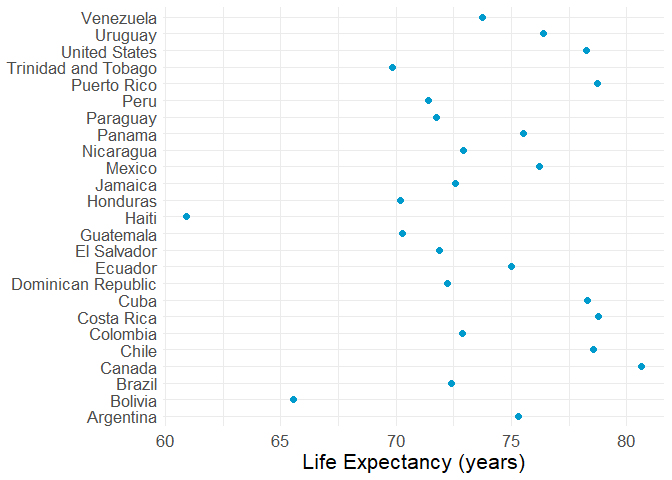
\includegraphics{PerceptionAndVisualization_files/figure-latex/unnamed-chunk-2-1.pdf}

\hypertarget{with-some-adjustments-the-basic-plot-can-be-brought-close-to-the-gapminder-version-in-appearance}{%
\paragraph{2. With some adjustments the basic plot can be brought close
to the Gapminder version in
appearance:}\label{with-some-adjustments-the-basic-plot-can-be-brought-close-to-the-gapminder-version-in-appearance}}

\begin{Shaded}
\begin{Highlighting}[]
\NormalTok{gm2007 }\OtherTok{\textless{}{-}} \FunctionTok{filter}\NormalTok{(gapminder, year }\SpecialCharTok{==} \DecValTok{2007}\NormalTok{) }\SpecialCharTok{|\textgreater{}}
  \FunctionTok{arrange}\NormalTok{(}\FunctionTok{desc}\NormalTok{(pop)) }\DocumentationTok{\#\# Sort to avoid over{-}plotting}
\FunctionTok{ggplot}\NormalTok{(gm2007) }\SpecialCharTok{+}
  \FunctionTok{geom\_point}\NormalTok{(}\FunctionTok{aes}\NormalTok{(}\AttributeTok{x =}\NormalTok{ gdpPercap,}
                 \AttributeTok{y =}\NormalTok{ lifeExp,}
                 \AttributeTok{size =}\NormalTok{ pop,}
                 \AttributeTok{fill =}\NormalTok{ continent),}
             \AttributeTok{shape =} \DecValTok{21}\NormalTok{) }\SpecialCharTok{+} \DocumentationTok{\#\# to allow the using \textquotesingle{}fill\textquotesingle{} aesthetic}
  \FunctionTok{scale\_x\_log10}\NormalTok{() }\SpecialCharTok{+}
  \FunctionTok{ylim}\NormalTok{(}\FunctionTok{c}\NormalTok{(}\DecValTok{20}\NormalTok{, }\DecValTok{85}\NormalTok{)) }\SpecialCharTok{+}
  \FunctionTok{scale\_size\_area}\NormalTok{(}\AttributeTok{max\_size =} \DecValTok{20}\NormalTok{,}
                  \AttributeTok{labels =} \FunctionTok{waiver}\NormalTok{() ,}
                  \AttributeTok{breaks =} \FunctionTok{c}\NormalTok{(}\FloatTok{0.25} \SpecialCharTok{*} \DecValTok{10} \SpecialCharTok{\^{}} \DecValTok{9}\NormalTok{, }\FloatTok{0.5} \SpecialCharTok{*} \DecValTok{10} \SpecialCharTok{\^{}} \DecValTok{9}\NormalTok{, }\DecValTok{10} \SpecialCharTok{\^{}} \DecValTok{9}\NormalTok{)) }\SpecialCharTok{+}
  \FunctionTok{scale\_fill\_manual}\NormalTok{(}\AttributeTok{values =} \FunctionTok{c}\NormalTok{(}\AttributeTok{Africa =} \StringTok{"deepskyblue"}\NormalTok{,}
                               \AttributeTok{Asia =} \StringTok{"red"}\NormalTok{,}
                               \AttributeTok{Americas =} \StringTok{"green"}\NormalTok{,}
                               \AttributeTok{Europe =} \StringTok{"gold"}\NormalTok{,}
                               \AttributeTok{Oceania =} \StringTok{"brown"}\NormalTok{)) }\SpecialCharTok{+}
  \FunctionTok{labs}\NormalTok{(}\AttributeTok{x =} \StringTok{"Income"}\NormalTok{ , }\AttributeTok{y =} \StringTok{"Life Expectancy"}\NormalTok{) }\SpecialCharTok{+}
  \FunctionTok{theme}\NormalTok{(}\AttributeTok{text =} \FunctionTok{element\_text}\NormalTok{(}\AttributeTok{size =} \DecValTok{16}\NormalTok{)) }\SpecialCharTok{+}
  \FunctionTok{guides}\NormalTok{(}\AttributeTok{fill =} \FunctionTok{guide\_legend}\NormalTok{(}\AttributeTok{title =} \StringTok{"Continent"}\NormalTok{,}
                             \AttributeTok{override.aes =} \FunctionTok{list}\NormalTok{(}\AttributeTok{size =} \DecValTok{5}\NormalTok{), }\AttributeTok{order =} \DecValTok{1}\NormalTok{),}
         \AttributeTok{size =} \FunctionTok{guide\_legend}\NormalTok{(}\AttributeTok{title =} \StringTok{"Population"}\NormalTok{,}
                             \AttributeTok{label.hjust =} \DecValTok{1}\NormalTok{,}
                             \AttributeTok{order =} \DecValTok{2}\NormalTok{)) }\SpecialCharTok{+} 
  \FunctionTok{theme\_minimal}\NormalTok{() }\SpecialCharTok{+} 
  \FunctionTok{theme}\NormalTok{(}\AttributeTok{panel.border =} \FunctionTok{element\_rect}\NormalTok{(}\AttributeTok{fill =} \ConstantTok{NA}\NormalTok{, }\AttributeTok{color =} \StringTok{"grey20"}\NormalTok{))}
\end{Highlighting}
\end{Shaded}

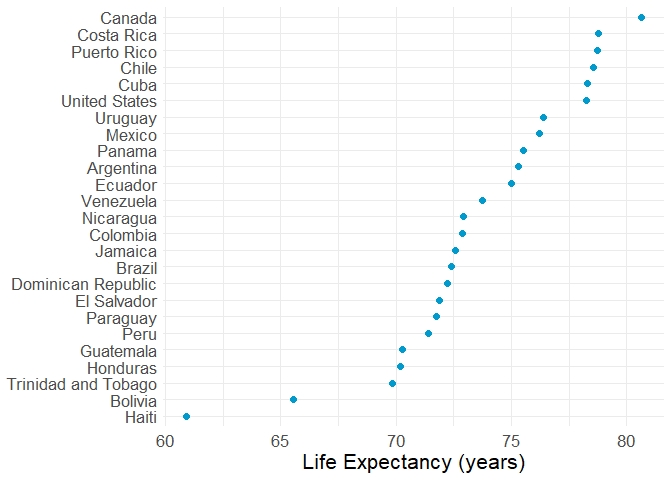
\includegraphics{PerceptionAndVisualization_files/figure-latex/unnamed-chunk-3-1.pdf}

\hypertarget{to-judge-the-marginal-association-between-life-expectancy-and-population-size-we-can-change-the-channel-mapping}{%
\paragraph{3. To judge the marginal association between life expectancy
and population size we can change the channel
mapping:}\label{to-judge-the-marginal-association-between-life-expectancy-and-population-size-we-can-change-the-channel-mapping}}

\begin{itemize}
\tightlist
\item
  map the horizontal axis to population;
\item
  map area to income.
\end{itemize}

\begin{Shaded}
\begin{Highlighting}[]
\NormalTok{gm2007 }\OtherTok{\textless{}{-}} \FunctionTok{filter}\NormalTok{(gapminder, year }\SpecialCharTok{==} \DecValTok{2007}\NormalTok{)}
\FunctionTok{ggplot}\NormalTok{(gm2007) }\SpecialCharTok{+}
  \FunctionTok{geom\_point}\NormalTok{(}\FunctionTok{aes}\NormalTok{(}\AttributeTok{x =}\NormalTok{ pop,}
                 \AttributeTok{y =}\NormalTok{ lifeExp,}
                 \AttributeTok{size =}\NormalTok{ gdpPercap)) }\SpecialCharTok{+}
  \FunctionTok{scale\_x\_log10}\NormalTok{() }\SpecialCharTok{+}
  \FunctionTok{ylim}\NormalTok{(}\FunctionTok{c}\NormalTok{(}\DecValTok{20}\NormalTok{, }\DecValTok{85}\NormalTok{)) }\SpecialCharTok{+}
  \FunctionTok{theme\_minimal}\NormalTok{() }\SpecialCharTok{+}
  \FunctionTok{theme}\NormalTok{(}\AttributeTok{panel.border =} \FunctionTok{element\_rect}\NormalTok{(}\AttributeTok{fill =} \ConstantTok{NA}\NormalTok{,}
                                    \AttributeTok{color =} \StringTok{"grey20"}\NormalTok{))}
\end{Highlighting}
\end{Shaded}

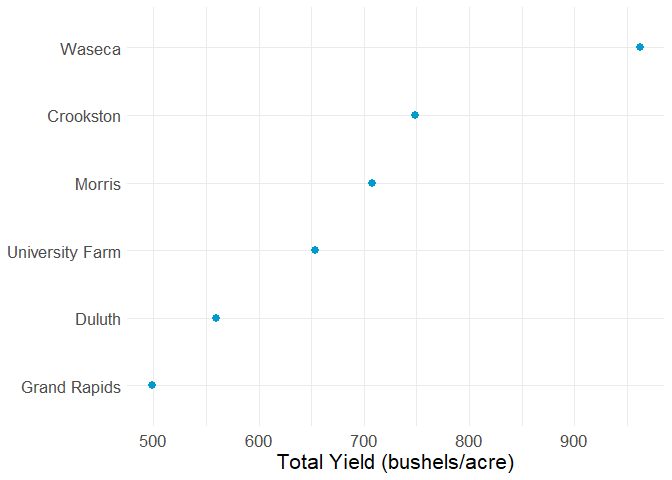
\includegraphics{PerceptionAndVisualization_files/figure-latex/unnamed-chunk-4-1.pdf}

\end{document}
